\documentclass[11pt]{article}
\usepackage[fontsize = 12pt]{scrextend}
\usepackage{multicol}
\usepackage{multirow}
\usepackage{savesym}
\usepackage{hyperref}
\usepackage{amsmath}
\usepackage{algorithm}
\usepackage{algorithmic}
\usepackage{paralist}
\usepackage{float}
\usepackage{bm}
\usepackage[shortlabels]{enumitem}
\usepackage[bb=px]{mathalpha}
\usepackage[a4paper, margin=1in]{geometry}
\usepackage[dvipsnames]{xcolor}
\usepackage{tikz}
\newtheorem{theorem}{Theorem}
\usetikzlibrary{shapes,backgrounds}
\usetikzlibrary{positioning}
\title{SDS 383C - Statistical Modeling 1: Homework 5}
\author{Rahul Nandakumar \\ Graduate Student, ORIE Program (E-ID: rn9355)}
\date{December 3, 2022}
\begin{document}
\maketitle
\noindent \textbf{\emph{1.}}\\ \\
\textbf{Solution:}\\ \\
We are given the true posterior of a parameter $\theta$ as $p(\theta \text{ }|\text{ } data) \equiv t_{3}(\theta)$.
\begin{figure}[H]
  \centering
  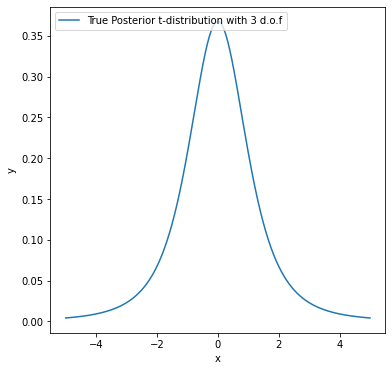
\includegraphics[width = 0.5\textwidth]{1a.png}
  \caption{True Posterior t-distribution with 3 d.o.f}
\end{figure}
\noindent \emph{a.} We now implement importance resampling in Python with the normal distribution as the reference density. Here, our density of interest is the t-distribution with 3 degrees of freedom which is hard to sample from. We have the standard normal distribution which is easy to sample from. We calculate the weights of the sample as the ratio between the pdf of the t distribution with 3 d.o.f and the standard normal distribution with each sample. After normalizing these weights, we resample from the original sample with probabilities given by the normalized weights. This process is importance resampling. The Python code is attached with this assignment and the results are displayed below. We carry out this resampling process for a 100 and 10000 samples in 2 separate simulations. Our observation is that as the number of samples increases, we are able to better sample from the posterior distribution as evident from the fitting of the true posterior with the histogram.
\begin{figure}[H]
  \centering
  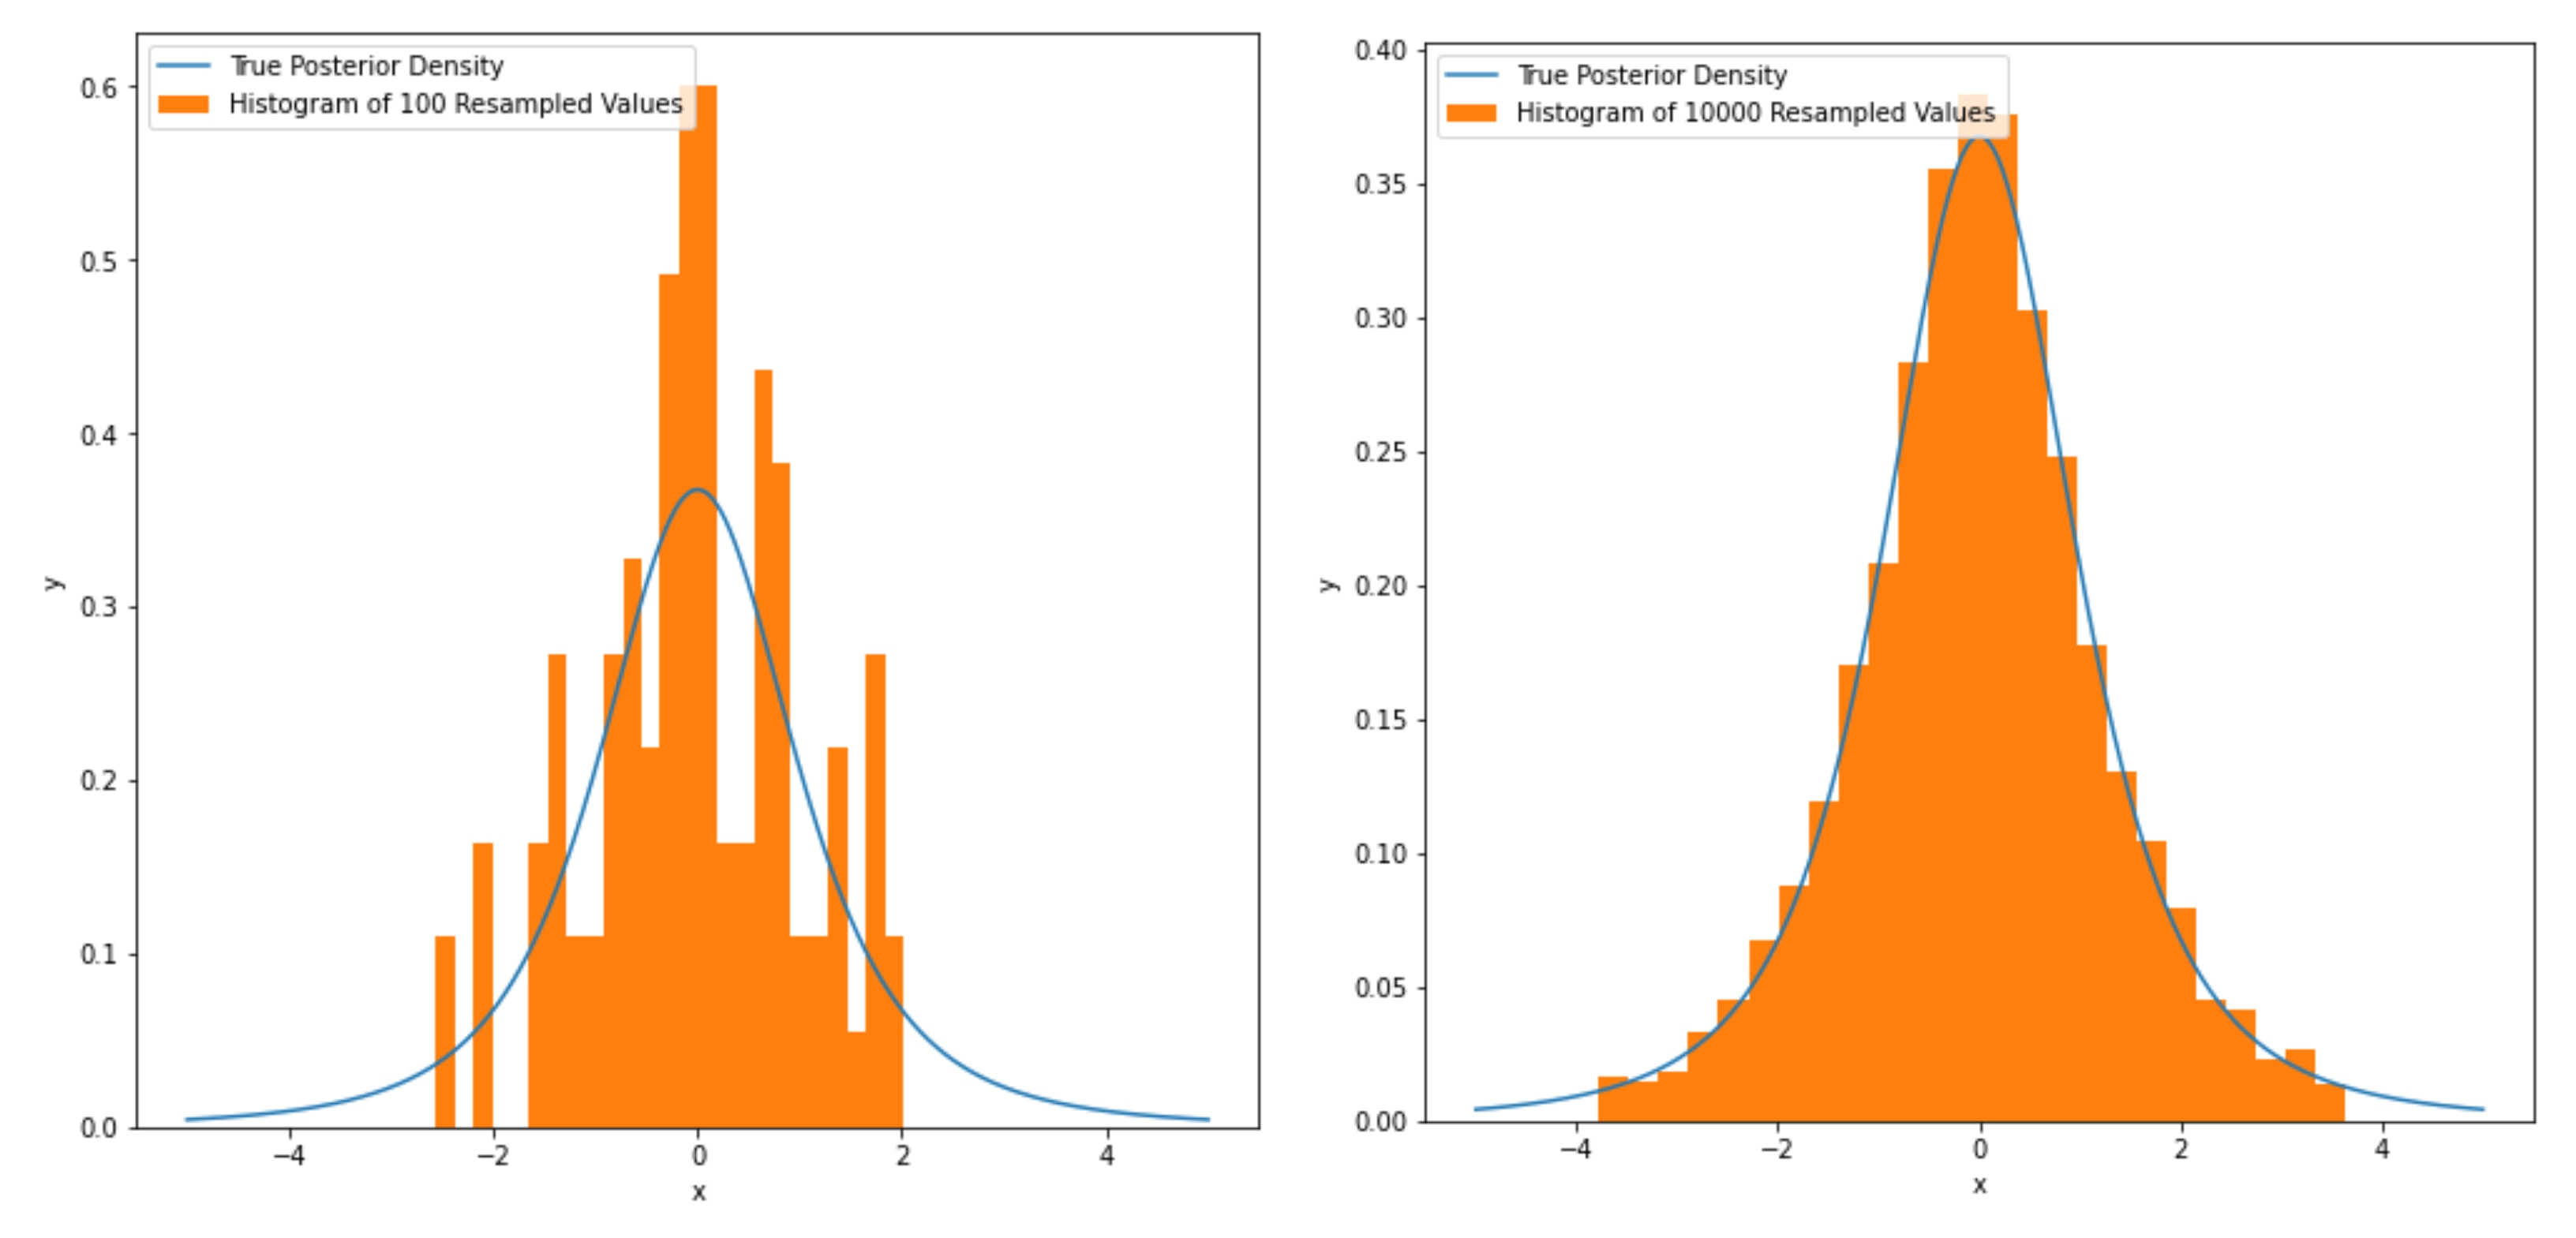
\includegraphics[width = 1\textwidth]{Importance Resampling Plots.jpg}
  \caption{Importance resampling for 100 and 10000 samples}
\end{figure}
\noindent \emph{b.} Importance sampling is similar in implementation to importance resampling, except here we donot resample from the original sample using the normalized weights as the probabilities of picking each sample. Instead, importance sampling can be used to calculate other useful parameters such as the mean and the variance of a given sample, which can be used to estimate the true mean and variance of the distribution. Our implementation is same as in importance resampling, where we find the weights as the ratio between the pdf of the t distribution with 3 d.o.f and the standard normal distribution with each sample. We then normalize these weights. Now, the mean of the samples is calculated as the sum-product of the weights and samples, and the variance is calculated as the sum-product of the weights and the square of the difference between the sample value and the sample calculated previously. This is implemented in Python and the results are as follows. The estimated mean for 100 samples is evaluated as $0.3838500475232623$, and the estimated variance for 100 samples is estimated as $1.9797163514580358$. The estimated mean for 10000 samples evaluates to $0.012160083789871339$ and the estimated variance for 10000 evaluates to $2.842751834188354$. The true mean of the t-distribution is 0 and the true variance of theh t-distribution with $v$ d.o.f is given by $\frac{v}{v-2} (= \frac{3}{1} = 3 \text{ in our case})$. We observe as the number of samples increase, we are able to better predict the true mean and variance.\\ \\
\textbf{\emph{2.}} \\ \\
\textbf{\emph{Solution}}\\ \\
We are given a bivariate normal distribution with the following parameters.
\begin{equation}
  \nonumber
  \begin{aligned}
    (\mu_{1}, \mu_{2}) & = (0,2)\\
    (\sigma_{1}^{2}, \sigma_{2}^{2}) & = (1,1)\\
    \rho & = 0.75\\
  \end{aligned}
\end{equation}
We are asked to construct a Gibbs Sampler that draws samples from this bivariate normal distribution. Using the value of $\rho$, we can construct the covariance matrix using the relation,
\begin{equation}
  \nonumber
  \begin{aligned}
    \rho & = \frac{Cov(X, Y)}{var(X) \times var(Y)}\\
    Cov(X, Y) & = 0.75
  \end{aligned}
\end{equation}
Therefore,
\begin{equation}
  \nonumber
  \begin{aligned}
    \Sigma & = \begin{bmatrix}
      var(X) & Cov(X, Y)\\
      Cov(X, Y) & var(Y)
      \end{bmatrix}
      & =  \begin{bmatrix}
        1 & 0.75\\
        0.75 & 1
        \end{bmatrix}
  \end{aligned}
\end{equation}
Using this covariance matrix and the means, we implement the Gibbs Sampler. The implementation has been carried out in R for the reason to obtain the autocorrelation plots and the contour plots with ease. We carry out the sampling for 1000 burned-in and thinned samples,
The results are as follows, and the R file is attached along with this assignment.
\begin{figure}[H]
  \centering
  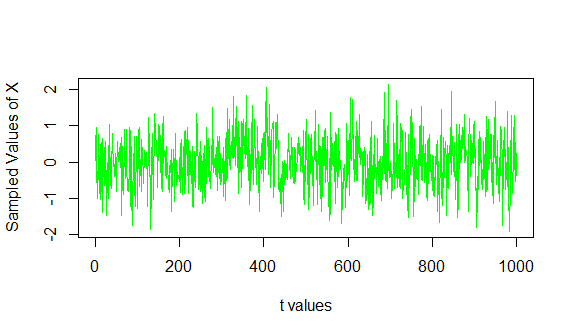
\includegraphics[width = 0.6\textwidth]{gibbs1-2.png}
  \caption{Traceplot Gibbs Sampled values of X}
\end{figure}
\begin{figure}[H]
  \centering
  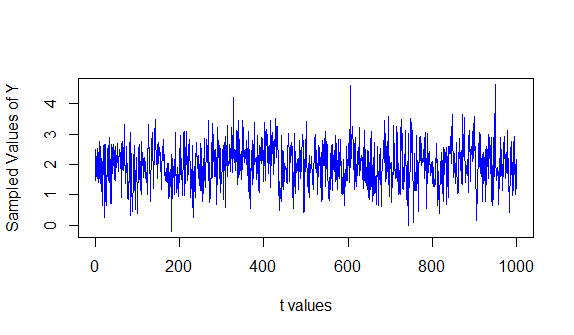
\includegraphics[width = 0.6\textwidth]{gibbs2-2.png}
  \caption{Traceplot Gibbs Sampled values of Y}
\end{figure}
\begin{figure}[H]
  \centering
  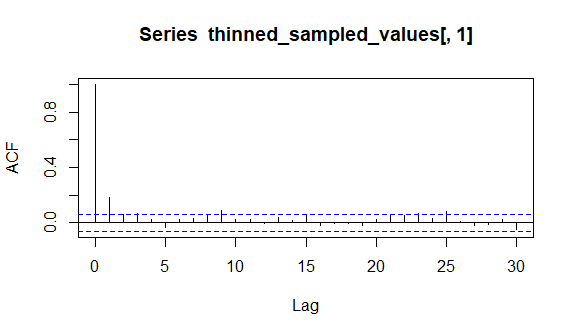
\includegraphics[width = 0.6\textwidth]{ACF-1.png}
  \caption{Autocorrelation plot for X}
\end{figure}
\begin{figure}[H]
  \centering
  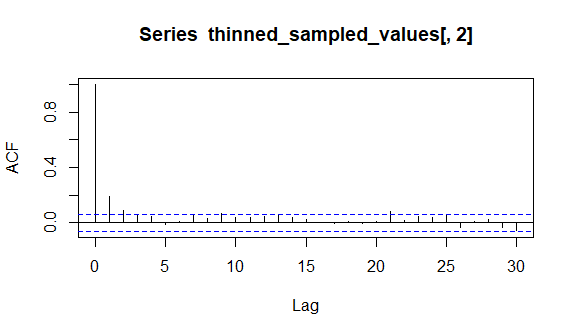
\includegraphics[width = 0.6\textwidth]{ACF-2.png}
  \caption{Autocorrelation Plot for Y}
\end{figure}
\begin{figure}[H]
  \centering
  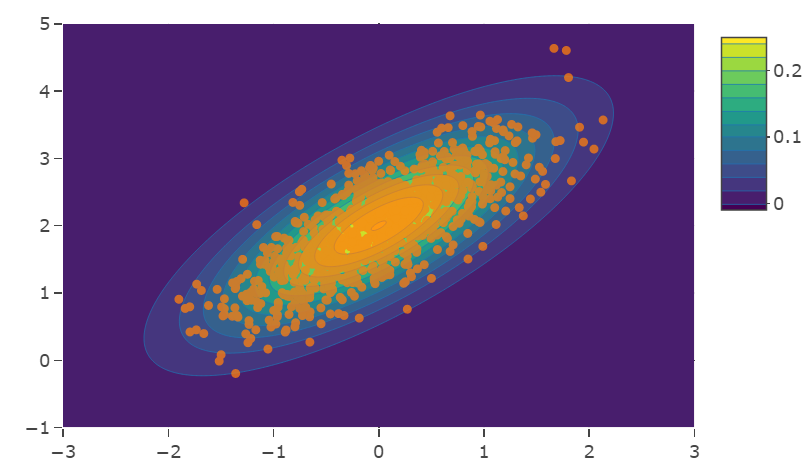
\includegraphics[width = 0.8\textwidth]{ContourPlot-2.png}
  \caption{Contour Plot of actual density superimposed over sampled values}
\end{figure}
\pagebreak
\noindent \textbf{\emph{3.}}\\ \\
\textbf{Solution:}\\ \\
We are given an AR(1) process with mean $\mu$, correlation $|\rho| < 1$ and error variance $\sigma^2$ which evolves as follows.
\begin{equation}
  \nonumber
  \begin{aligned}
    y_{t} & = \mu + \rho(y_{t-1} -\mu) + \epsilon_{t}
  \end{aligned}
\end{equation}
Where $\epsilon_{t} \text{ iid  with } \mathbb{E}(\epsilon_t) = 0 \text{ and var }(\epsilon_t) = \sigma^2$. Here, we understand that $\mathbb{E}(y_{t}) = \mu$ \\ \\
\emph{a.} We know that
\begin{equation}
  \nonumber
  \begin{aligned}
    var(y_{t}) & = \mathbb{E}(y_{t}^{2}) - \mathbb{E}(y_{t})^{2}\\
    & = \mathbb{E}(y_{t}(\mu + \rho(y_{t-1} -\mu) + \epsilon_{t})) - \mu^2\\
    & = \mathbb{E}(y_{t}(\mu(1-\rho))) + \rho\mathbb{E}(y_{t}y_{t-1}) + \mathbb{E}(y_{t}\epsilon_{t}) - \mu^2\\
    & = (\mu(1-\rho))\mathbb{E}(y_{t})+ \rho\mathbb{E}(y_{t}y_{t-1}) + \mathbb{E}(y_{t}\epsilon_{t}) - \mu^2\\
    & = (\mu(1-\rho))\mathbb{E}(y_{t})+ \rho(Cov(y_{t}, y_{t-1}) + \mathbb{E}(y_{t})\mathbb{E}(y_{t-1})) + \mathbb{E}(y_{t}\epsilon_{t}) - \mu^2\\
    & = \rho^{2}var(y_{t}) + \sigma^2\\
    var(y_{t})(1-\rho^2) &= \sigma^2\\
    var(y_{t}) & = \frac{\sigma^2}{(1-\rho^2)}
  \end{aligned}
\end{equation}
\emph{b.} Let us consider
\begin{equation}
  \nonumber
  \begin{aligned}
    y_{t} & = \mu + \rho(y_{t-1} -\mu) + \epsilon_{t}\\
    y_{t} & = \mu(1- \rho) + \rho(y_{t-1}) + \epsilon_{t}\\
    y_{t} & = \rho(y_{t-1}) + A_{t}; \text{ Let }\mu(1- \rho) +\epsilon_{t} =  A_{t}\\
    y_{t-k}y_{t} & = \rho(y_{t-1})y_{t-k} + A_{t}y_{t-k}; \text{ Multiplying both sides by }y_{t-k}\\
    \mathbb{E}(y_{t-k}y_{t}) & = \rho\mathbb{E}((y_{t-1})y_{t-k}) + \mathbb{E}(A_{t}y_{t-k}); \text{ Taking expectation of this expression}\\
  \end{aligned}
\end{equation}
Let us denote the covariance of $y_{t}$ and $y_{t-k}$ by $\gamma_{k}$. Now,
\begin{equation}
  \nonumber
  \begin{aligned}
    \gamma_{k} & = \rho\gamma_{k-1}\\
    \gamma_{k} & = \rho^{k}\gamma_{0}; \text{ Going recursively to } \gamma_{0} \text{ from }\gamma_{k-1}\\
  \end{aligned}
\end{equation}
From this relation, we can say that
\begin{equation}
  \nonumber
  \begin{aligned}
    corr(y_{t}, y_{t-k}) & = \frac{\gamma_{k}}{var(y_{t})var(y_{t-k})}\\
    & = \frac{\rho^{k}\gamma_{0}}{var(y_{t})var(y_{t-k})}\\
    & = \rho^{k}\\
  \end{aligned}
\end{equation}
\emph{c.}\\ \\
We know that,
\begin{equation}
  \nonumber
  y_{t} = \mu + \rho(y_{t-1} -\mu) + \epsilon_{t}
\end{equation}
Now,
\begin{equation}
  \nonumber
  \begin{aligned}
    \mathbb{E}(\bar{y}_{n}) & = \mathbb{E}\bigg(\frac{y_{1} + y_{2} + \dots y_{n}}{n}\bigg)\\
    & = \frac{1}{n}(\mathbb{E}(y_{1}) + \dots \mathbb{E}(y_{n}))\\
    & = \frac{1}{n}(n \mu)\\
    & = \mu
  \end{aligned}
\end{equation}
\emph{d.}\\ \\
\emph{e.} We know from the previous result that
\begin{equation}
  \nonumber
  \begin{aligned}
    var(\bar{y}_{n}) & = \frac{\sigma^2}{n^{2}(1-\rho^2)}\bigg(n+2\sum_{j=1}^{n-1}(n-j)\rho^j\bigg)\\
    n\text{var}(\bar{y}_{n}) & = \frac{\sigma^2}{n(1-\rho^2)}\bigg(n+2\sum_{j=1}^{n-1}(n-j)\rho^j\bigg); \text{ Multiplying both sides with n}\\
    & = \frac{\sigma^2}{(1-\rho^2)}\bigg(1+2\sum_{j=1}^{n-1}(1-\frac{j}{n})\rho^j\bigg)\\
    & = \frac{\sigma^2}{(1-\rho^2)}\bigg(1+2(\rho + \rho^2 + \dots +\infty)\bigg); \text{ Since } n \rightarrow \infty, \frac{1}{n} \rightarrow 0\\
    & = \frac{\sigma^2}{(1-\rho^2)}\bigg(1+2\bigg(\frac{\rho}{1-\rho}\bigg)\bigg); \text{ Sum of infinite G.P.}\\
    & = \frac{\sigma^2}{(1-\rho^2)}\bigg(\frac{1+\rho}{1-\rho}\bigg)\\
    n\text{var}(\bar{y}_{n}) & =  \frac{\sigma^2}{(1-\rho)^2}
  \end{aligned}
\end{equation}
\emph{f.} \\ \\
Now,
\begin{equation}
  \nonumber
  \begin{aligned}
    \mathbb{E}(s_n^2) & = \mathbb{E}\bigg(\frac{n-1}{n}s^2\bigg) \\
    & =  \mathbb{E}\bigg(1-\frac{1}{n}s^2\bigg)\\
    & = \bigg(1-\frac{1}{n}\bigg)\mathbb{E}(s^2)\\
  \end{aligned}
\end{equation}
As $n \rightarrow \infty$, $\frac{1}{n} \rightarrow 0$ and $\mathbb{E}(s^2) \rightarrow \text{var}(y_{t})$. Therefore, we can conclude that as $n \rightarrow \infty$
\begin{equation}
  \nonumber
  \begin{aligned}
    \mathbb{E}(s_n^2) \rightarrow \text{var}(y_{t})
  \end{aligned}
\end{equation}
\textbf{\emph{4.}}\\ \\
We are given a AR(1) process and we are asked to simulate 500 points from this process for analysis. The process has mean $\mu = 0$, correlation $\rho = 0.75$ and Normally distributed errors with $\sigma^2 = 1$. Now, we fit a Bayesian Model to this data points.\\ \\
\emph{a.}
Our given process is,
\begin{equation}
  \nonumber
  y_{t} = \rho y_{t-1} + e_{t}
\end{equation}
This implies that our model can also be written as,
\begin{equation}
  \nonumber
  f(y_{t} \text{ }| \text{ } y_{t-1}, \rho, \sigma^2) \sim \text{Normal}(\rho y_{t-1}, \sigma^2)
\end{equation}
The likelihood function for this model can be written as
\begin{equation}
  \nonumber
  \begin{aligned}
    p(y_{1:n} \text{ } | \text{ } \mu, \sigma^2) &= \prod_{i = 2}^{t}f(y_{i} \text{ }| \text{ } y_{i-1}, \rho, \sigma^2)\\
    & = \prod_{i = 2}^{t}\text{Normal}(\rho y_{i-1}, \sigma^2)\\
    & = (2\pi\sigma^2)^{\frac{-(n-1)}{2}}\text{exp}\bigg(\frac{-1}{2\sigma^2}\sum_{i = 2}^{t}(y_{i} - \rho y_{i-1})^2\bigg)\\
  \end{aligned}
\end{equation}
From this likelihood, we can estimate the priors of our model as having a conjugate NIG prior. Mathematically, it is expressed as,
\begin{equation}
  \nonumber
  \begin{aligned}
    p(\rho \text{ }|\text{ } \sigma^2) & = \text{Normal}\bigg(\mu_{0}, \frac{\sigma^2}{k_{0}}\bigg)\\
    p(\sigma^2) & = \text{Inverse-Gamma}\bigg(\frac{v_{0}}{2}, \frac{v_{0}\sigma_{0}^2}{2}\bigg)
  \end{aligned}
\end{equation}
\emph{b.} Under these conjugate priors, we can obtain the full conditionals as follows. First, we evaluate the posterior.
\begin{equation}
  \nonumber
  \begin{aligned}
    p(\rho, \sigma^2 | y_{1:n}) & = p(\rho, \sigma^2)\times p(y_{1:n}|\rho, \sigma^2)\\
    & = (2\pi\sigma^2)^{\frac{-(n-1)}{2}}\text{exp}\bigg(\frac{-1}{2\sigma^2}\sum_{t = 2}^{n}(y_{t} - \rho y_{t-1})^2\bigg) \times p(\rho \text{ }|\text{ } \sigma^2) \times p(\sigma^2)\\
    & = (2 \pi \sigma^2)^{-(\frac{v_0+1}{2})-1}\text{exp}\bigg(\frac{-1}{2\sigma^2}(v_{0}\sigma_0^2 + \kappa_{0}\rho^2)\bigg) \times (2\pi\sigma^2)^{\frac{-(n-1)}{2}}\text{exp}\bigg(\frac{-1}{2\sigma^2}\sum_{t = 2}^{n}(y_{t} - \rho y_{t-1})^2\bigg)\\
    & \propto (\sigma^2)^{\frac{-(v_0 + n)}{2}-1}\text{exp}{\frac{-1}{2\sigma^2}\bigg(v_0\sigma_0^2 + (\rho-\rho_n)^2\kappa_n - \kappa_n\rho_n^2 + \sum_{t=2}^{n}y_{t}^2\bigg)}\\
  \end{aligned}
\end{equation}
This is the kernel of an NIG Distribution with parameters $(\rho_n, \kappa_n, v_n, \sigma_n^2)$. Here, we have the hyperparameters equal to
\begin{equation}
  \nonumber
  \begin{aligned}
    \kappa_n &= \kappa_0 + \sum_{t=2}^{n}y_{t-1}^2\\
    \rho_n &= \frac{1}{\kappa_n}\bigg(\sum_{t=2}^{n}y_{t}y_{t-1}\bigg)\\
    \sigma_n^2 &= \frac{1}{2}\bigg(v_0\sigma_0^2-\kappa_n\rho_n^2 + \sum_{t=2}^{n}y_t^2\bigg)\\
    v_n & = v_0 + n - 1
  \end{aligned}
\end{equation}
From this kernel, we can obtain the full conditionals for $\rho$ and $\sigma^2$ by assuming either one of the parameters are given. This gives us,
\begin{equation}
  \nonumber
  \begin{aligned}
    p(\rho \text{ } | \text{ } \sigma^2, y_{1:n}) & = \text{Normal}\bigg(\rho, \frac{\sigma^2}{\kappa_n}\bigg)\\
    p(\sigma^2 \text{ } | \text{ } \rho, y_{1:n}) & = \text{Inverse-Gamma}\bigg(\frac{v_n}{2}, \frac{2\sigma_n^2+\kappa_n(\rho-\rho_n)^2}{2}\bigg)
  \end{aligned}
\end{equation}
\emph{c.} Now, we implement the Gibbs sampler in R by using these full conditionals. First, we simulate 500 points from this process with parameters mean $\mu = 0$, correlation $\rho = 0.75$. We also choose suitable values for the hyperparameters as shown in the R Code. We generate 10000 samples initially, from which we burn in the samples by removing the first 2000 samples and we thin the samples by a factor of 4. This gives us 2000 burned-in and thinned gibbs samples from which we can estimate the values of $\rho$ and $\sigma^2$. The R code is attached with this assignment and the traceplot is attached below.
\begin{figure}[H]
  \centering
  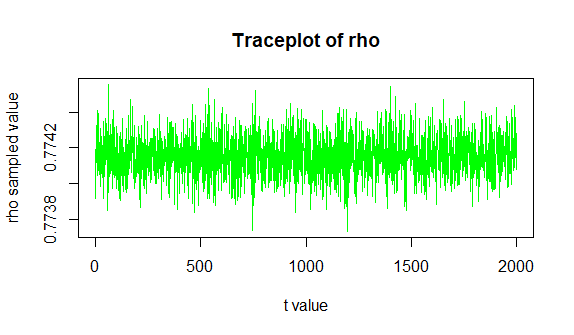
\includegraphics[width = 0.7\textwidth]{4-1.png}
  \caption{Traceplot for Gibbs sampled values of $\rho$}
\end{figure}
\begin{figure}[H]
  \centering
  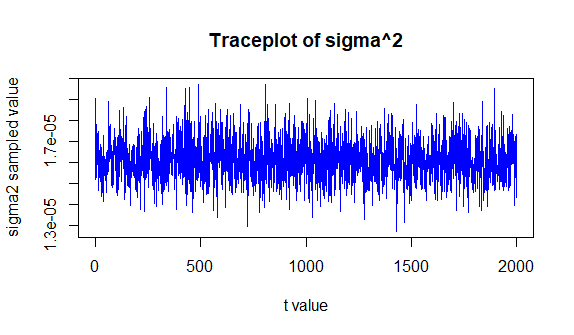
\includegraphics[width = 0.7\textwidth]{4-2.png}
  \caption{Traceplot for Gibbs sampled values of $\sigma^2$}
\end{figure}
\noindent After the sampling process, the final values of $\rho$ and $\sigma^2$ equals 0.7742298 and 1.579148e-05 respectively. \\ \\
\emph{d.} Now, we construct the 90\% credible intrevals for $\rho$ and $\sigma^2$. We do this in R, using the Quantile based credible intrevals, as it was mentioned in the lecture notes that Quantile based credible intrevals are used much more in practice. It is defined as,
\begin{equation}
  \nonumber
  \begin{aligned}
    C_{\theta, \alpha} & = \{\theta : Pr(C_{\theta, \alpha \text{ }|\text{ } y_{1:n}}) = 1 - \alpha\}\\
    & = \{\theta_{n, 1 - \alpha_{1}} \leq \theta \leq \theta_{n, \alpha_{2}}, \alpha_{1} + \alpha_{2} = \alpha\}
  \end{aligned}
\end{equation}
Implementing this in R, we get, mean lower bound = $0.694460081689918$ and mean upper bound = $0.694460082861651$ and variance lower bound = $1.42763850294374 \times 10^{-05}$ and variance upper bound = $1.427638503367 \times 10^{-05}$\\ \\
\textbf{\emph{5.}}\\ \\
\textbf{\emph{Solution:}} We are given a normal mixture normal model to fit to the galaxies dataset in R. This dataset consists of velocities in km/sec of 82 galaxies from 6 well-separated conic sections of an unfilled survey of the Corona Borealis region. We desire to fit a normal location - scale mixture model of the form
\begin{equation}
  \nonumber
  y_{i} \overset{iid}{\sim} \sum_{k = 1}^{K} \pi_{k} \text{Normal}(y_{i} \text{ } | \text{ } \mu_{k}, \sigma_{k}^2)
\end{equation}
We are given priors for this model as follows.
\begin{equation}
  \nonumber
  \begin{aligned}
    \bm{\pi} & \sim \text{Dir}(1/K, . . . , 1/K)\\
    \mu_k & \sim \text{Normal}(\mu_0, \sigma_0^2)\\
    \sigma_k^2 & \sim \text{Inverse-Gamma}(a_0, b_0)
  \end{aligned}
\end{equation}
We need to sample $z, \mu_k, \sigma_k^2$. We can get the full conditionals as follows,
\begin{equation}
  \nonumber
  \begin{aligned}
    p(z_{i} = k | \dots) & = \text{Mult}(1, \bm{\pi}), \pi_{ik} = \frac{\pi_k \times \text{Normal}(y_i | \mu_k, \sigma_k^2)}{\sum_{j=1}{K}\pi_j \times \text{Normal}(y_i | \mu_j, \sigma_j^2)}\\
    p(\mu_k | \dots)  & = \text{Normal}(\mu_{k,n}, \sigma_{k,n}^2), \mu_{k,n} = \sigma_{k,n}^2\bigg(\frac{\mu_0}{\sigma_0^2} + \frac{n_k\bar{y}_k}{\sigma_k^2}\bigg), \sigma_{k,n}^2 = \bigg(\frac{1}{\sigma^2} + \frac{n_k}{\sigma_k^2}\bigg)^{-1}\\
    & \text{where, }n_{k} = \sum_{i}1(z_{i} = k), \bar{y}_{k} = \frac{\sum_{i}1(z_{i} = k)y_{i}}{n_k}\\
    p(\sigma_k^2 | \dots) & = \text{Inv-Gamma}(a_{k,n}, b_{k,n})\\
    & a_{k,n} = (a_0 + \frac{n_k}{2}), b_{k,n} = \bigg(b_0 + \frac{(n_k-1)s_k^2}{2} + \frac{n_k(\bar{y}_k - \mu_k)}{2}\bigg)
  \end{aligned}
\end{equation}
We implement the gibbs sampler in R by sampling from these conditional distributions. For the pointwise credible region, we calculate them using the idea illustrated in question 4. We calculate the upper and lower bound for each point using the values of these credible regions at each point. The R file containing this results has been attached along with this assignment.
\begin{figure}[H]
  \centering
  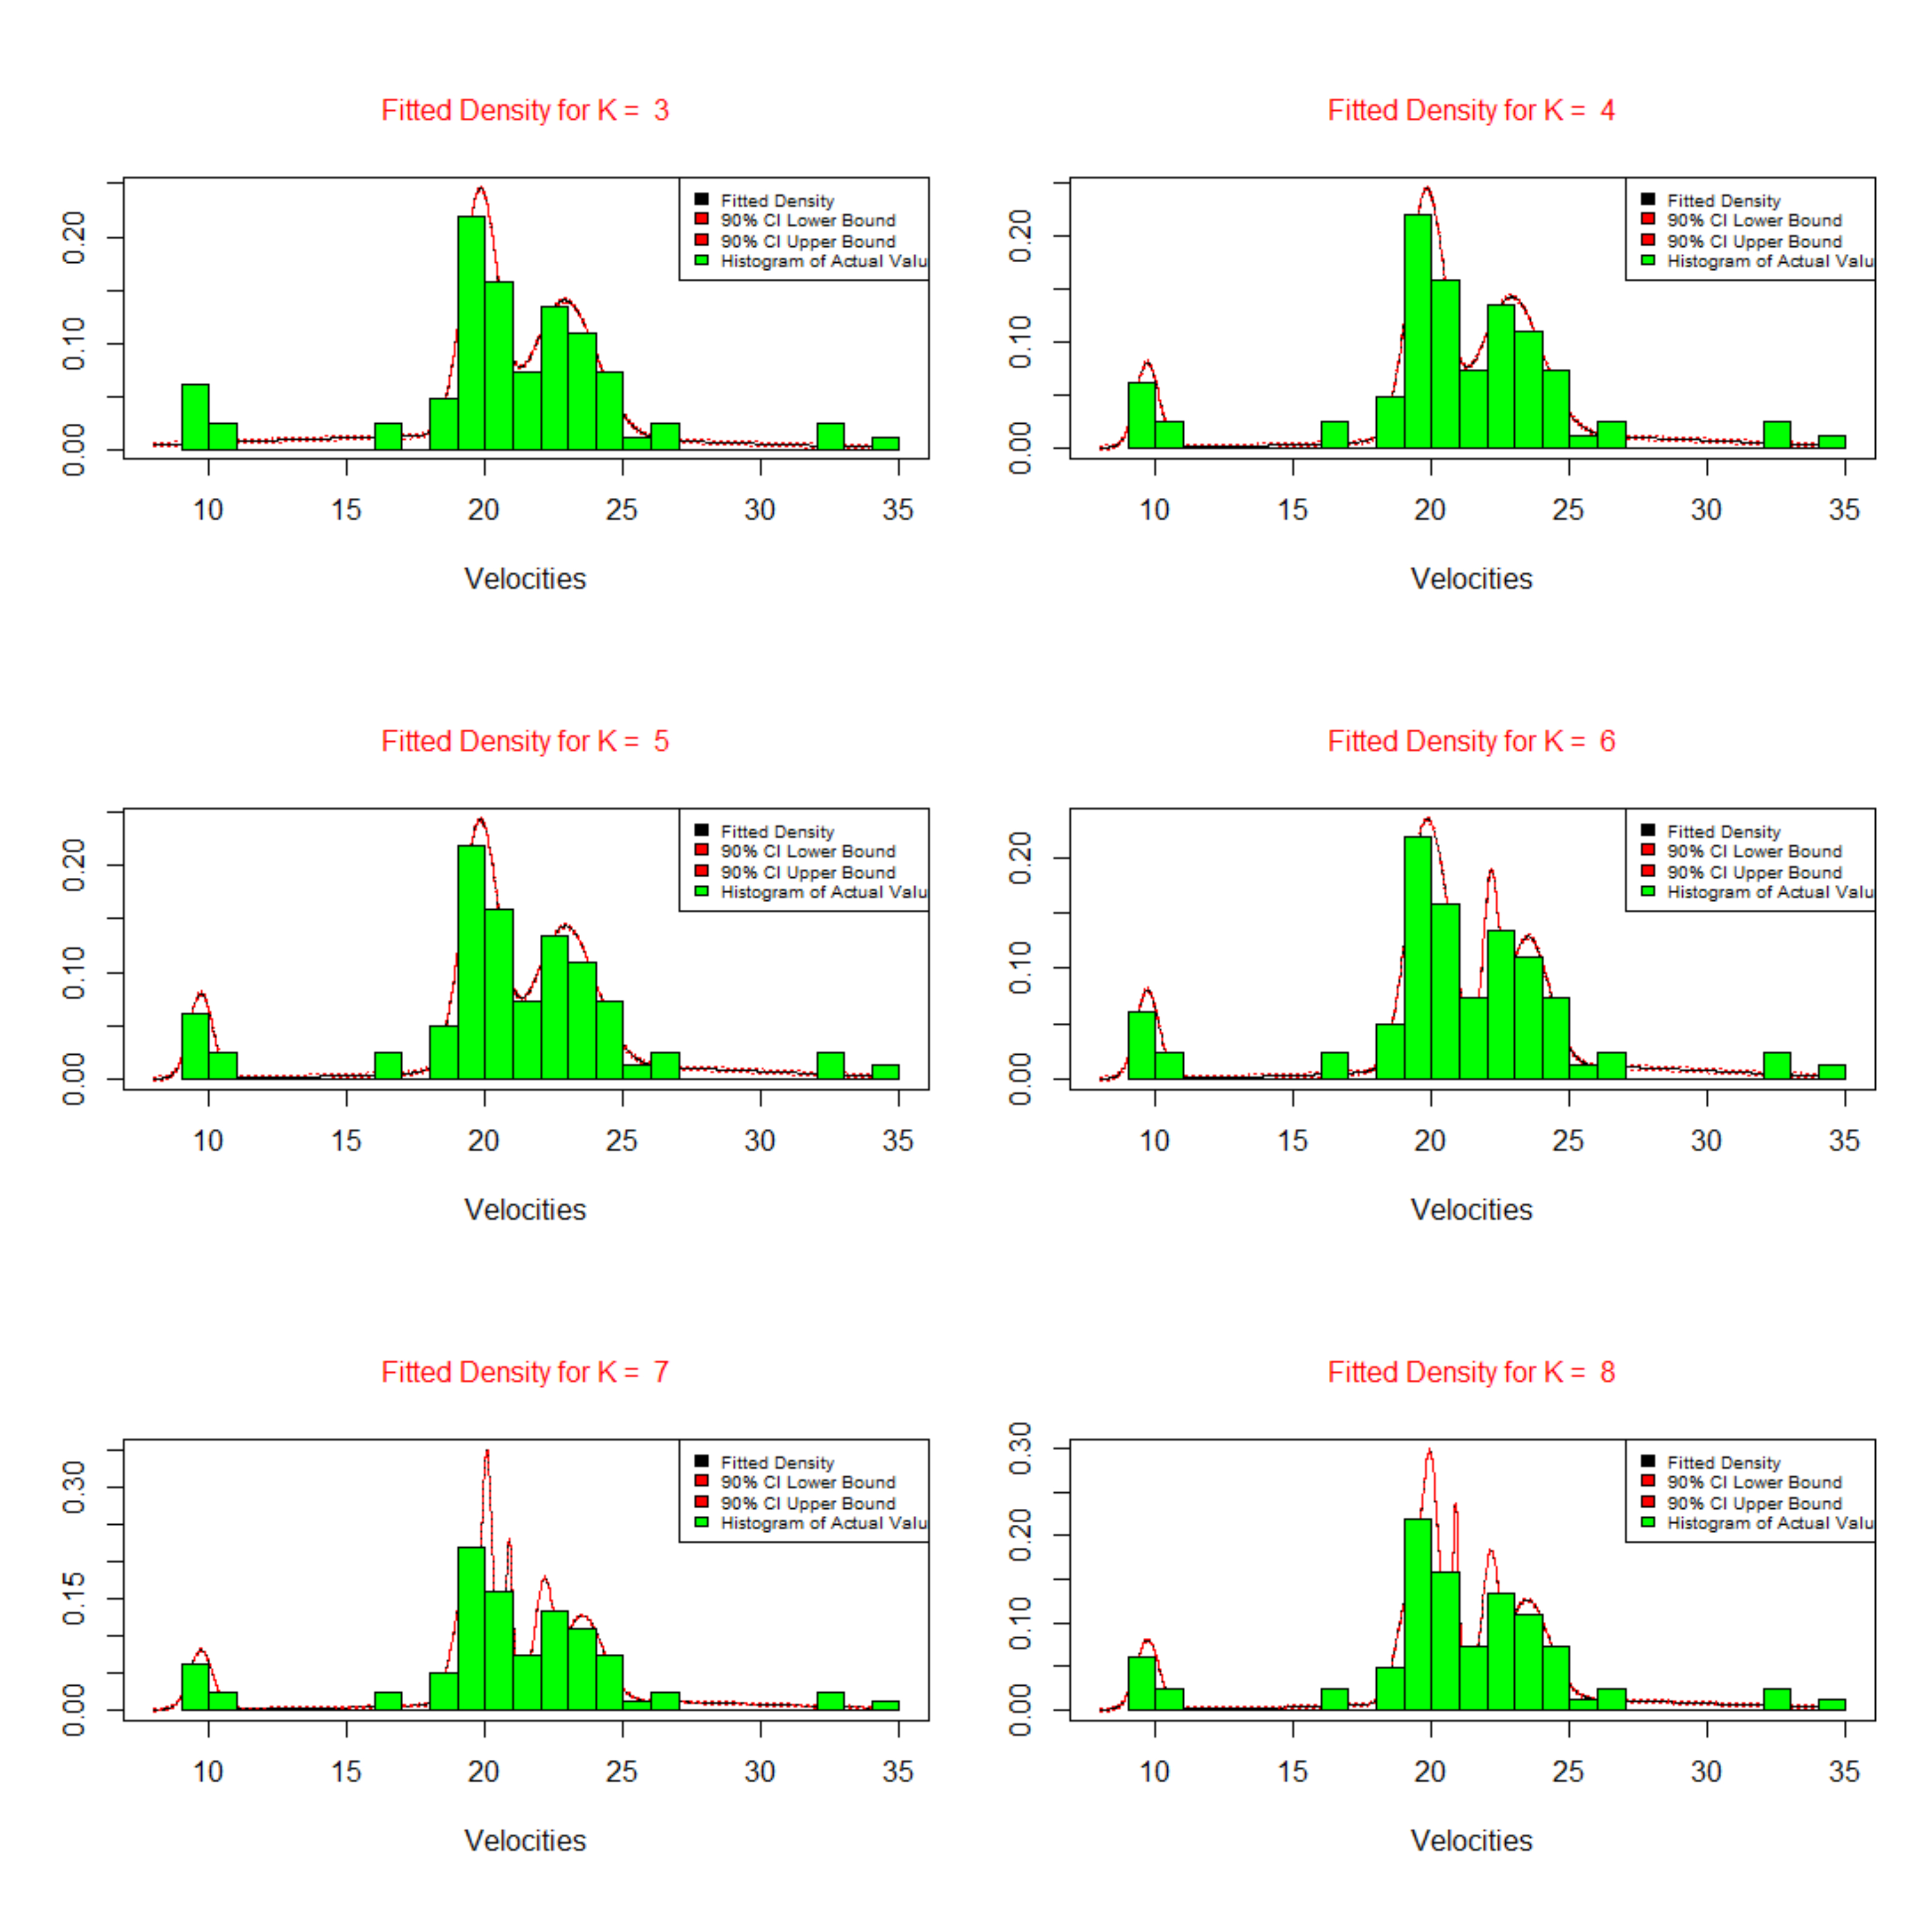
\includegraphics[width = 1\textwidth]{Fitted Densities.jpg}
  \caption{Plot of Fitted Densities, Credible Intrevals and Histogram of sample values}
\end{figure}
\noindent \textbf{\emph{6.}}\\ \\
\textbf{\emph{Solution:}} In this problem, we are given a bivariate normal mixture model to fit to the faithful dataset in R. The dataset consists of the waiting times between eruptions and the duration of the eruption for the Old Faithful geyser in Yellowstone National Park, Wyoming, USA. We desire to fit a Multivariate Normal Mixture Distribution with $K$ componenets of the form
\begin{equation}
  \nonumber
  \mathbf{y}_{1}, \dots, \mathbf{y}_{n} \overset{iid}{\sim} \sum_{k = 1}^{K} \pi_{k}\text{MVN}(\bm{\mu}_{k}, \bm{\Sigma}_{k})
\end{equation}
Where the priors are given as follows,
\begin{equation}
  \nonumber
  \begin{aligned}
    \bm{\pi} & \sim \text{Dir}(1/k,\dots,1/k)\\
    \bm{\mu}_k & \sim \text{Multivariate - Normal}(\bm{\mu}_{0}, \bm{\Sigma_{0}})\\
    \bm{\Sigma_{k}} & \sim \text{Inverse - Wishart}(v_{0}, \bm{\Psi}_{0})
  \end{aligned}
\end{equation}
Now, from the posterior distributions, we obtain the following full conditionals.
\begin{equation}
  \nonumber
  \begin{aligned}
    p(\bm{\pi} \text{ } | \text{ } \dots) & = \text{Dir}(\alpha/k,\dots,\alpha/k)\\
    p(\bm{\mu}_k \text{ } | \text{ } \dots) & = \text{Normal}(\bm{\mu}_{k,n}, \bm{\Sigma}_{k,n}^2)\\
    \text{where }\bm{\mu}_{k,n} & = \bm{\Sigma}_{k,n}(\bm{\mu}_0\bm{\Sigma}_{0}^{-1} + n_k\bar{y}_k\bm{\Sigma}_{k}^{-1}),\\
    \bm{\Sigma}_{k,n} & = (\bm{\Sigma}_{0}^{-1} + n_k\bm{\Sigma}_{k}^{-1})^{-1}\\
    p(\bm{\Sigma}_{k} \text{ }|\text{ } \dots) & = \text{Inverse-Wishart}(v_{k,n}, \psi_{k,n})\\
    \text{where } v_{k,n} & = v_0 + n_k, \\
    \psi_{k,n} &= \psi_0 + \sum_{z_{i} = k}(y_i-\mu_k)(y_i-\mu_k)^{T}
  \end{aligned}
\end{equation}
We implement the gibbs sampler in R by sampling from these conditional distributions and resuse the code from the previous assigment to plot the contour plots. We generate a contour plot by sampling from 100 values of x between 0.1 and 0.6 and y between 0.3 and 1. Here, we note that we worked with scaled down values of eruptions and waiting time, that is, we divide all eruptions by 10 and all waiting times by 100. The results are as shown below. The R file containing this results has been attached along with this assignment.
\begin{figure}[H]
  \centering
  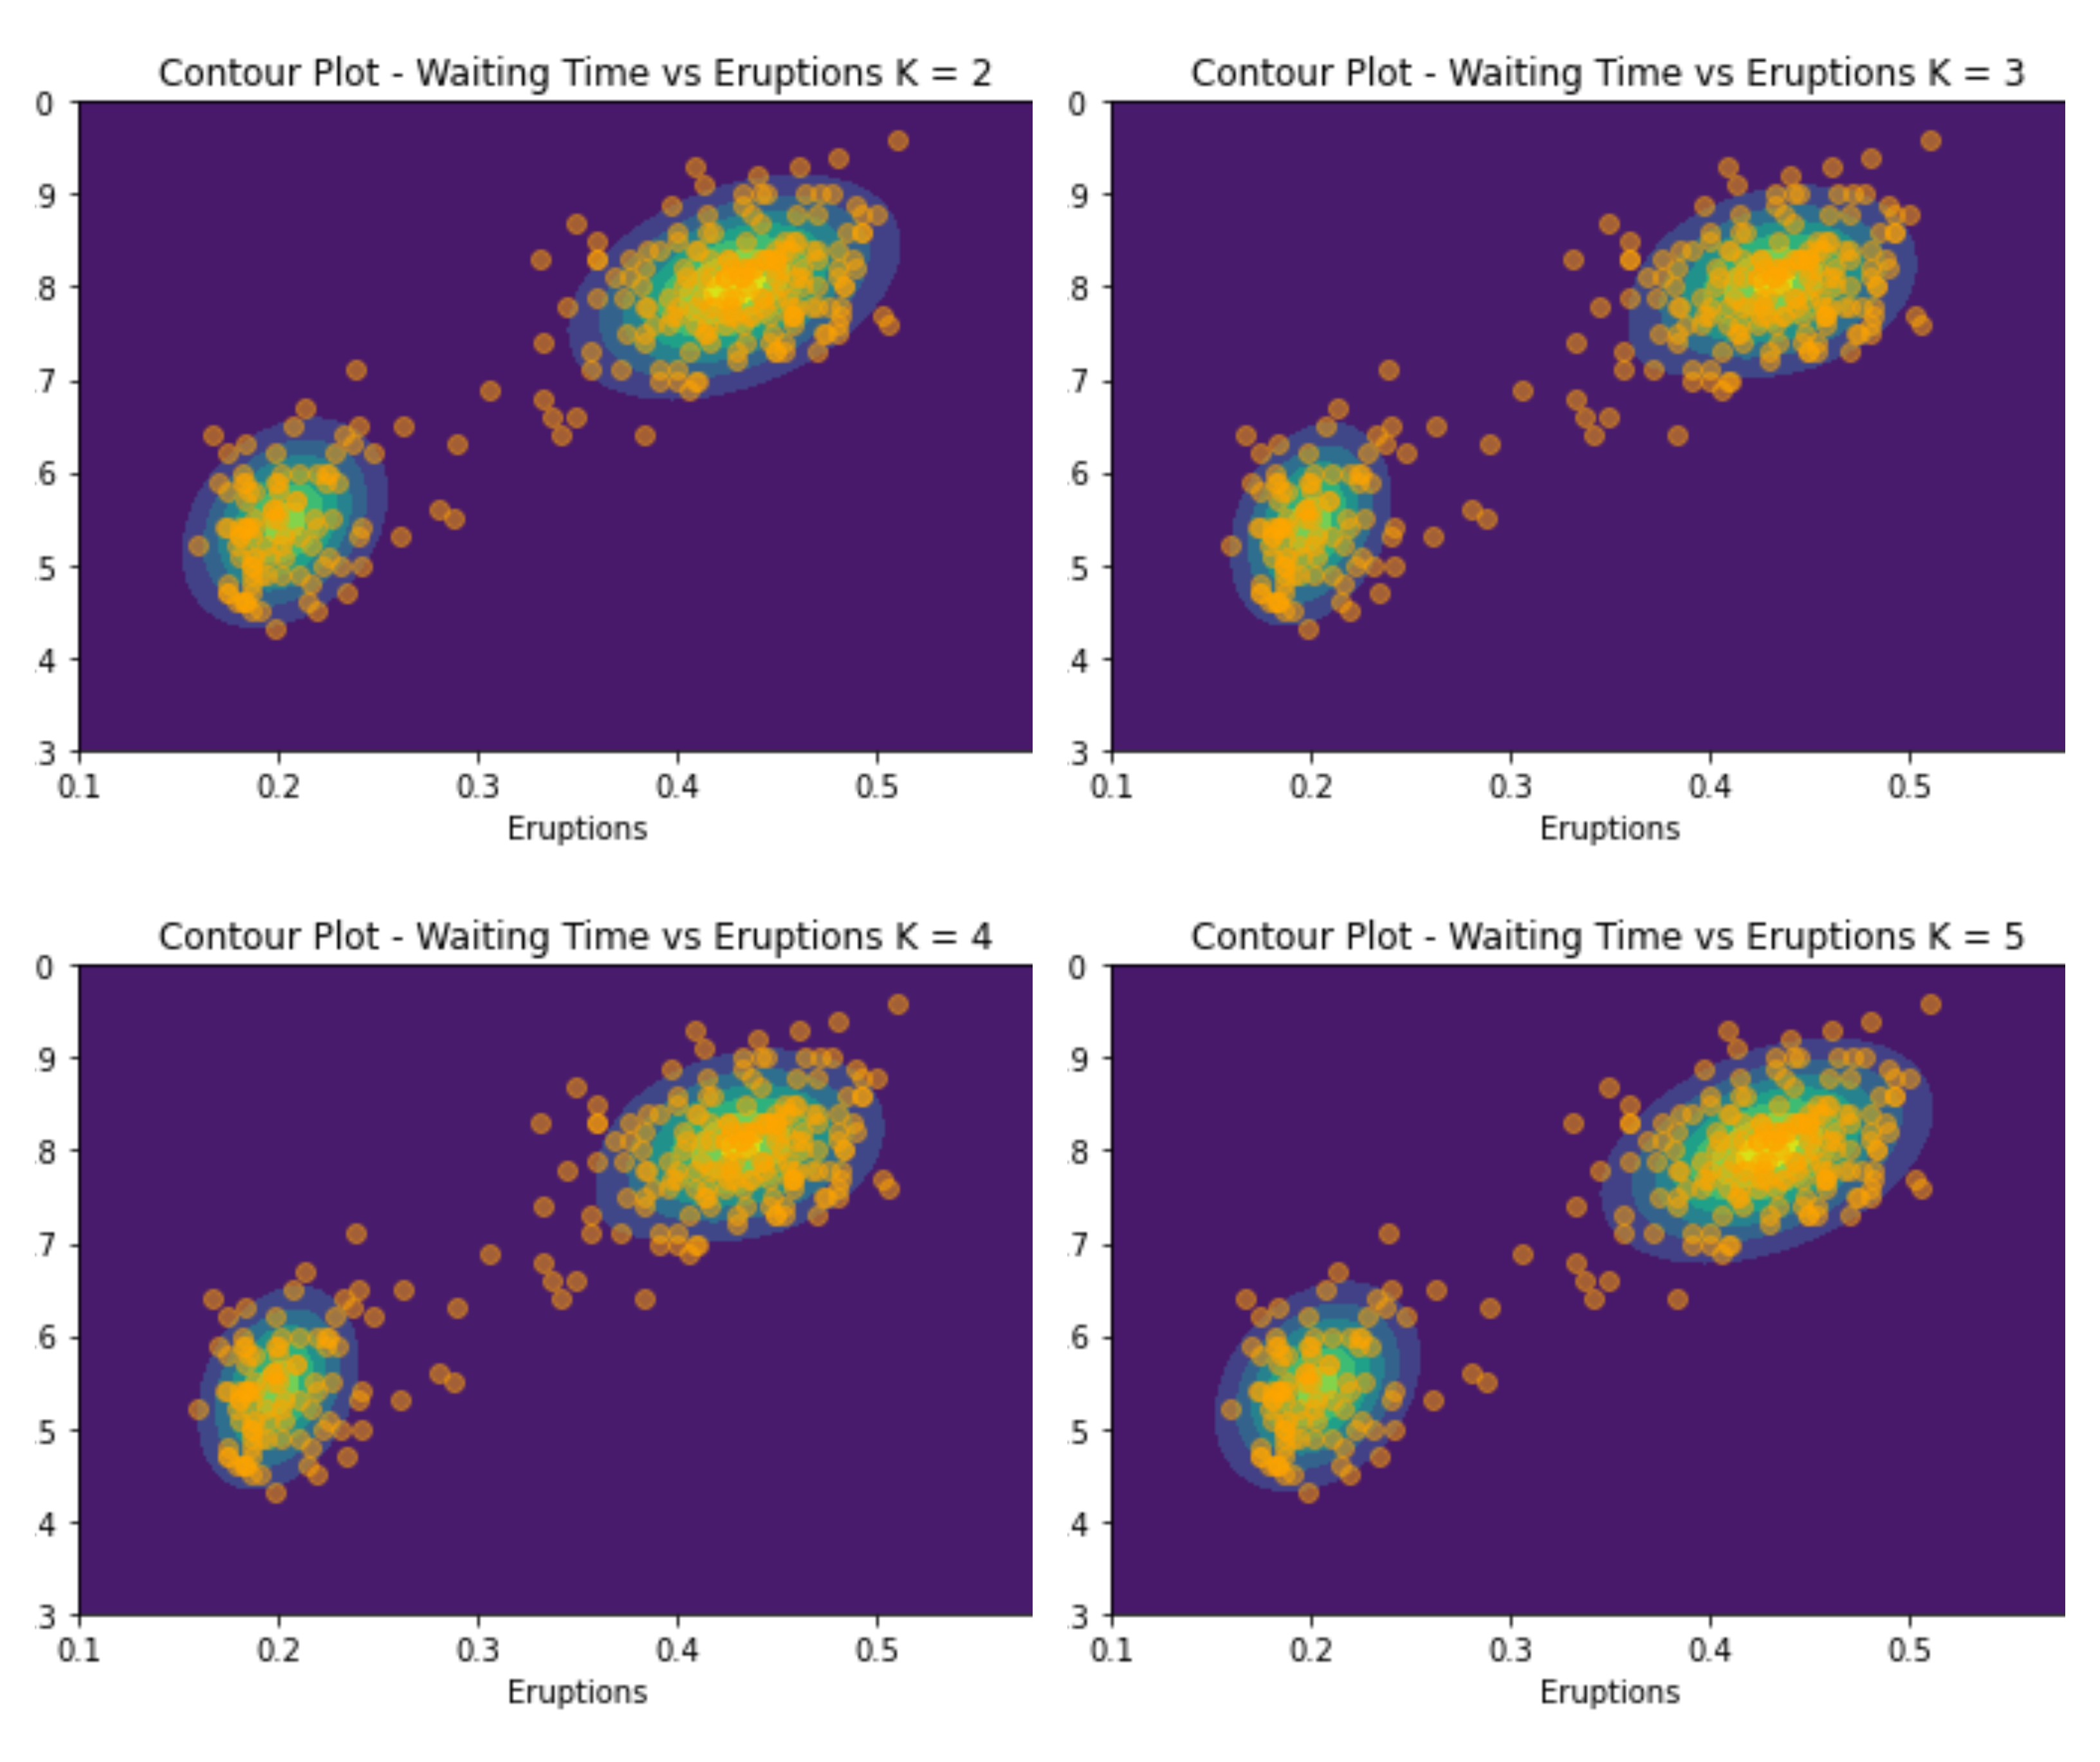
\includegraphics[width = 0.8\textwidth]{6plots.jpg}
  \caption{Contour plots superimposed over actual data distribution}
\end{figure}
\end{document}
